%% LyX 2.3.4.2 created this file.  For more info, see http://www.lyx.org/.
%% Do not edit unless you really know what you are doing.
\documentclass[english,dvipsnames,aspectratio=169]{beamer}
\usepackage{mathptmx}
\usepackage{eulervm}
\usepackage[T1]{fontenc}
\usepackage[latin9]{inputenc}
\usepackage{babel}
\usepackage{amstext}
\usepackage{amssymb}
\usepackage{graphicx}
\usepackage{ifthen}
\usepackage{xcolor}
\usepackage{xspace}
\usepackage{tikz}
\usetikzlibrary{tikzmark}
\usetikzlibrary{calc}
\usepackage{pgfplots}
%\pgfplotsset{compat=1.17}
\usepackage{booktabs}
\usepackage{xpatch}

\xpatchcmd{\itemize}
  {\def\makelabel}
  {\ifnum\@itemdepth=1\relax
     \setlength\itemsep{2ex}% separation for first level
   \else
     \ifnum\@itemdepth=2\relax
       \setlength\itemsep{1ex}% separation for second level
     \else
       \ifnum\@itemdepth=3\relax
         \setlength\itemsep{0.5ex}% separation for third level
   \fi\fi\fi\def\makelabel
  }
 {}
 {}

\ifx\hypersetup\undefined
  \AtBeginDocument{%
    \hypersetup{unicode=true,pdfusetitle,
 bookmarks=true,bookmarksnumbered=false,bookmarksopen=false,
 breaklinks=false,pdfborder={0 0 0},pdfborderstyle={},backref=false,colorlinks=true,
 allcolors=NYUPurple,urlcolor=LightPurple}
  }
\else
  \hypersetup{unicode=true,pdfusetitle,
 bookmarks=true,bookmarksnumbered=false,bookmarksopen=false,
 breaklinks=false,pdfborder={0 0 0},pdfborderstyle={},backref=false,colorlinks=true,
 allcolors=NYUPurple,urlcolor=LightPurple}
\fi

\makeatletter

%%%%%%%%%%%%%%%%%%%%%%%%%%%%%% LyX specific LaTeX commands.
%% Because html converters don't know tabularnewline
\providecommand{\tabularnewline}{\\}

%%%%%%%%%%%%%%%%%%%%%%%%%%%%%% Textclass specific LaTeX commands.
% this default might be overridden by plain title style
\newcommand\makebeamertitle{\frame{\maketitle}}%
% (ERT) argument for the TOC
\AtBeginDocument{%
  \let\origtableofcontents=\tableofcontents
  \def\tableofcontents{\@ifnextchar[{\origtableofcontents}{\gobbletableofcontents}}
  \def\gobbletableofcontents#1{\origtableofcontents}
}

%%%%%%%%%%%%%%%%%%%%%%%%%%%%%% User specified LaTeX commands.
\usetheme{CambridgeUS} 
\beamertemplatenavigationsymbolsempty


% Set Color ==============================
\definecolor{NYUPurple}{RGB}{87,6,140}
\definecolor{LightPurple}{RGB}{165,11,255}


\setbeamercolor{title}{fg=NYUPurple}
\setbeamercolor{frametitle}{fg=NYUPurple}

\setbeamercolor{background canvas}{fg=NYUPurple, bg=white}
\setbeamercolor{background}{fg=black, bg=NYUPurple}

\setbeamercolor{palette primary}{fg=black, bg=gray!30!white}
\setbeamercolor{palette secondary}{fg=black, bg=gray!20!white}
\setbeamercolor{palette tertiary}{fg=gray!20!white, bg=NYUPurple}

\setbeamertemplate{headline}{}
\setbeamerfont{itemize/enumerate body}{}
\setbeamerfont{itemize/enumerate subbody}{size=\normalsize}

\setbeamercolor{parttitle}{fg=NYUPurple}
\setbeamercolor{sectiontitle}{fg=NYUPurple}
\setbeamercolor{sectionname}{fg=NYUPurple}
\setbeamercolor{section page}{fg=NYUPurple}
%\setbeamercolor{description item}{fg=NYUPurple}
%\setbeamercolor{block title}{fg=NYUPurple}

\setbeamertemplate{blocks}[rounded][shadow=false]
\setbeamercolor{block body}{bg=normal text.bg!90!NYUPurple}
\setbeamercolor{block title}{bg=NYUPurple!30, fg=NYUPurple}



\AtBeginSection[]{
  \begin{frame}
  \vfill
  \centering
\setbeamercolor{section title}{fg=NYUPurple}
 \begin{beamercolorbox}[sep=8pt,center,shadow=true,rounded=true]{title}
    \usebeamerfont{title}\usebeamercolor[fg]{title}\insertsectionhead\par%
  \end{beamercolorbox}
  \vfill
  \end{frame}
}

\makeatother

\setlength{\parskip}{\medskipamount} 

\input ../macros

\begin{document}
\input ../rosenberg-macros

\title[DS-GA 1003]{Loss Functions}
\author{He He}
\date{Feb 9, 2021}
\institute{CDS, NYU}

\makebeamertitle
\mode<article>{Just in article version}

\begin{frame}
    {Review}
    Three spaces for a prediction problem:
    \begin{itemize}
        \item Input space $\sX$, e.g. email sender, title etc.
        \item Action space $\sA$, e.g. score of SPAM 
        \item Output space $\sY$, e.g. SPAM or NO SPAM
    \end{itemize}

    \medskip
\begin{block}{Loss Function}

A \textbf{loss function} evaluates an action in the context of the
outcome $y$.

\[
\begin{matrix}\loss: & \ca\times\cy & \rightarrow & \reals\\
& (a,y) & \mapsto & \loss(a,y)
\end{matrix}
\]
\end{block}
\end{frame}

\begin{frame}{Contents}
\tableofcontents{}
\end{frame}

\section{Regression Loss Functions}
\begin{frame}{Regression Problems}
\begin{itemize}
    \item Examples:
        \begin{itemize}
            \item Predicting the stock price given history prices
            \item Predicting medical cost of given age, sex, region, BMI etc.
            \item Predicting the age of a person based on their photos
        \end{itemize}

\item Regression spaces:
\begin{itemize}
\item Input space $\cx=\reals^{d}$
\item Action space $\ca=\reals$
\item Outcome space $\cy=\reals$.
\end{itemize}
\item Notation:
\begin{itemize}
\item $\hat{y}$ is the predicted value (the action)
\item $y$ is the actual observed value (the outcome)
\end{itemize}
\end{itemize}
\end{frame}
%
\begin{frame}{Loss Functions for Regression}

\begin{itemize}
\item In general, loss function may take the form
\[
\left(\hat{y},y\right)\mapsto\ell(\hat{y},y)\in\reals
\]


\item Regression losses usually only depend on the \textbf{residual $r=y-\hat{y}$.}

\begin{itemize}
\item what you have to add to your prediction to get the right answer
\end{itemize}

\item Loss $\ell(\hat{y},y)$ is called \textbf{distance-based }if it
\begin{enumerate}
\item only depends on the residual: 
\[
\ell(\hat{y},y)=\psi(y-\hat{y})\quad\text{for some \ensuremath{\psi}:\ensuremath{\reals\to\reals}}
\]


\item loss is zero when residual is $0$: 
\[
\psi(0)=0
\]
\end{enumerate}
\end{itemize}
\end{frame}
%
\begin{frame}{Distance-Based Losses are Translation Invariant}
\begin{itemize}
\item Distance-based losses are translation-invariant. That is,
\[
\ell(\hat{y}+b,y+b)=\ell\left(\hat{y},y\right)\qquad\forall b\in\reals.
\]

\item When might you not want to use a translation-invariant loss?

\pause{}
\item Sometimes relative error $\frac{\hat{y}-y}{y}$ is a more natural
loss (but not translation-invariant)

\item Often you can transform response $y$ so it's translation-invariant
(e.g. log transform)
\end{itemize}

\end{frame}

\begin{frame}{Some Losses for Regression}
\begin{itemize}
\item \textbf{Residual: $r=y-\hat{y}$}
\item \textbf{Square} or $\ell_{2}$ Loss: $\ell(r)=r^{2}$ 
\item \textbf{Absolute} or \textbf{Laplace} or $\ell_{1}$ Loss: $\ell(r)=\left|r\right|$ 
\end{itemize}

\begin{description}
\item [{%
\begin{tabular}{|c|c|c|c|}
\hline 
$y$ & $\hat{y}$ & $\left|r\right|=\left|y-\hat{y}\right|$ & $r^{2}=\left(y-\hat{y}\right)^{2}$\tabularnewline
\hline 
\hline 
1 & 0 & 1 & 1\tabularnewline
\hline 
5 & 0 & 5 & 25\tabularnewline
\hline 
10 & 0 & 10 & 100\tabularnewline
\hline 
50 & 0 & 50 & 2500\tabularnewline
\hline 
\end{tabular}}]~
\end{description}

\begin{itemize}
\item Outliers typically have large residuals.
\item Square loss much more affected by outliers than absolute loss.
\end{itemize}
\end{frame}

\begin{frame}{Loss Function Robustness}
\begin{itemize}
\item \textbf{Robustness }refers to how affected a learning algorithm is
by outliers.
\end{itemize}
\begin{center}
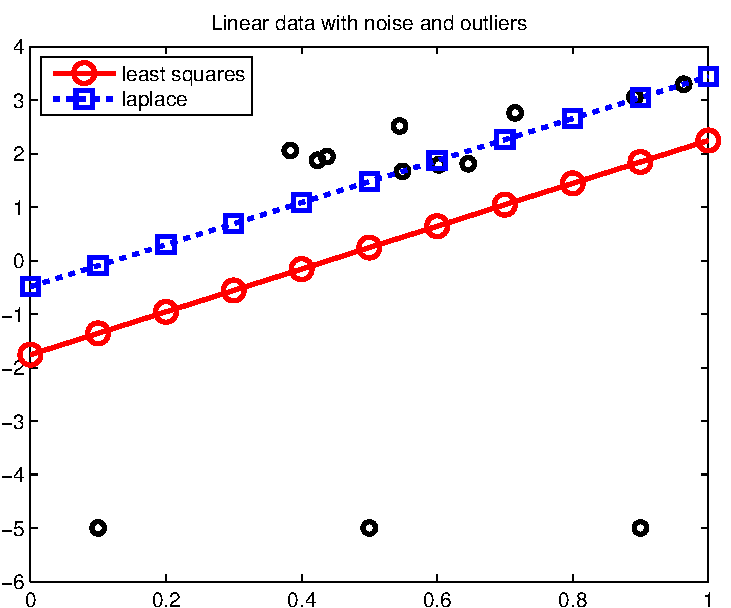
\includegraphics[height=0.6\textheight]{figures/fig7.6a}\let\thefootnote\relax\footnotetext{\tiny{KPM Figure 7.6}}
\par\end{center}

\end{frame}

\begin{frame}{Some Losses for Regression}

\let\thefootnote\relax\footnotetext{\tiny{KPM Figure 7.6}}
\begin{itemize}
\item \textbf{Square} or $\ell_{2}$ Loss: $\ell(r)=r^{2}$ (\emph{not robust})

\item \textbf{Absolute} or \textbf{Laplace} Loss: $\ell(r)=\left|r\right|$
(\emph{not differentiable})
\begin{itemize}
\item gives \textbf{median regression}
\end{itemize}

\item \textbf{Huber} Loss: Quadratic for $\left|r\right|\le\delta$ and
linear for $\left|r\right|>\delta$ (\emph{robust and differentiable})
    \begin{itemize}
    \item Equal values and slopes at $r=\delta$ 
    \end{itemize}
\end{itemize}
\begin{center}
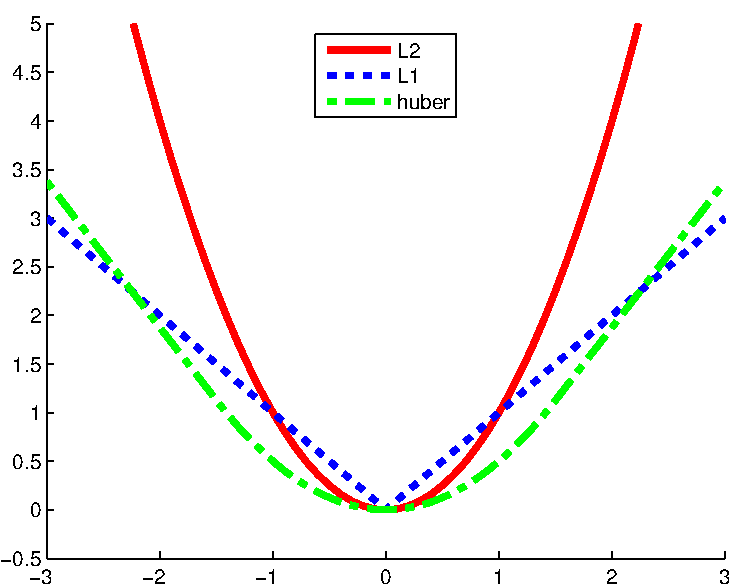
\includegraphics[height=0.4\textheight]{figures/fig7.6b}
\par\end{center}

\end{frame}


\section{Classification Loss Functions}

\begin{frame}{The Classification Problem}
    \begin{itemize}
    \item Examples:
        \begin{itemize}
            \item Predict whether the image contains a cat
            \item Predict whether the email is SPAM
        \end{itemize}

    \item Classification spaces:
    \begin{itemize}
        \item Input space $\reals^d$
        \item Action space $\ca=\reals$
        \item Outcome space $\cy=\left\{ -1,1\right\} $
    \end{itemize}
    \item Inference:
        \vspace{-2ex}
        \begin{itemize}
            \item[]
            \begin{align*}
            f(x)>0\;\implies & \mbox{Predict }1\\
            f(x)<0\;\implies & \mbox{Predict }-1
            \end{align*}
        \end{itemize}
    \end{itemize}
\end{frame}

\begin{frame}{The Score Function}
\begin{itemize}
\item Action space $\ca=\reals\qquad$ Output space $\cy=\left\{ -1,1\right\} $
\item \textbf{Real-valued prediction function} $f:\cx\to\reals$
\end{itemize}

\begin{definition}
The value $f(x)$ is called the \textbf{score} for the input $x$. 
\end{definition}

\begin{itemize}
\item In this context, $f$ may be called a \textbf{score function}.
\item Intuitively, magnitude of the score represents the \textbf{confidence
of our prediction}.
\end{itemize}
\end{frame}
%
\begin{frame}{The Margin}
\begin{definition}
The \textbf{margin} (or \textbf{functional margin})\textbf{ }for predicted
score $\hat{y}$ and true class $y\in\left\{ -1,1\right\} $ is $y\hat{y}$. 
\end{definition}


\begin{itemize}
\item The margin is often written as $yf(x)$, where $f(x)$ is our score function.

\item The margin is a measure of how \textbf{correct} we are.

\begin{itemize}
\item If $y$ and $\hat{y}$ are the same sign, prediction is \textbf{correct}
and margin is \textbf{positive}.
\item If $y$ and $\hat{y}$ have different sign, prediction is \textbf{incorrect}
and margin is \textbf{negative}.
\end{itemize}
    \item We want to \textbf{maximize the margin}
    \item Most classification losses depend only on the margin,
        which is called \textbf{margin-based loss}.
\end{itemize}
\end{frame}
%

\begin{frame}{Classification Losses: $0-1$ Loss}
\begin{itemize}
    \item \textbf{0-1 loss} for $f:\cx\to\left\{ -1,1\right\} $:
    \[
    \loss\left(f(x),y\right)=\ind{f(x)\neq y}
    \]
\item Empirical risk for $0-1$ loss:
\[
\hat{R}_{n}(f)=\frac{1}{n}\sum_{i=1}^{n}\ind{y_{i}f(x_{i})\leq0}
\]
\end{itemize}

\begin{alertblock}{Minimizing empirical $0-1$ risk not computationally feasible}

$\hat{R}_{n}(f)$ is non-convex, not differentiable (in fact, discontinuous!). 

Optimization is \textbf{NP-Hard}.
\end{alertblock}
\end{frame}

\begin{frame}{Classification Losses}

Zero-One loss: $\loss_{\text{0-1}}=\ind{m\le0}$
\begin{center}
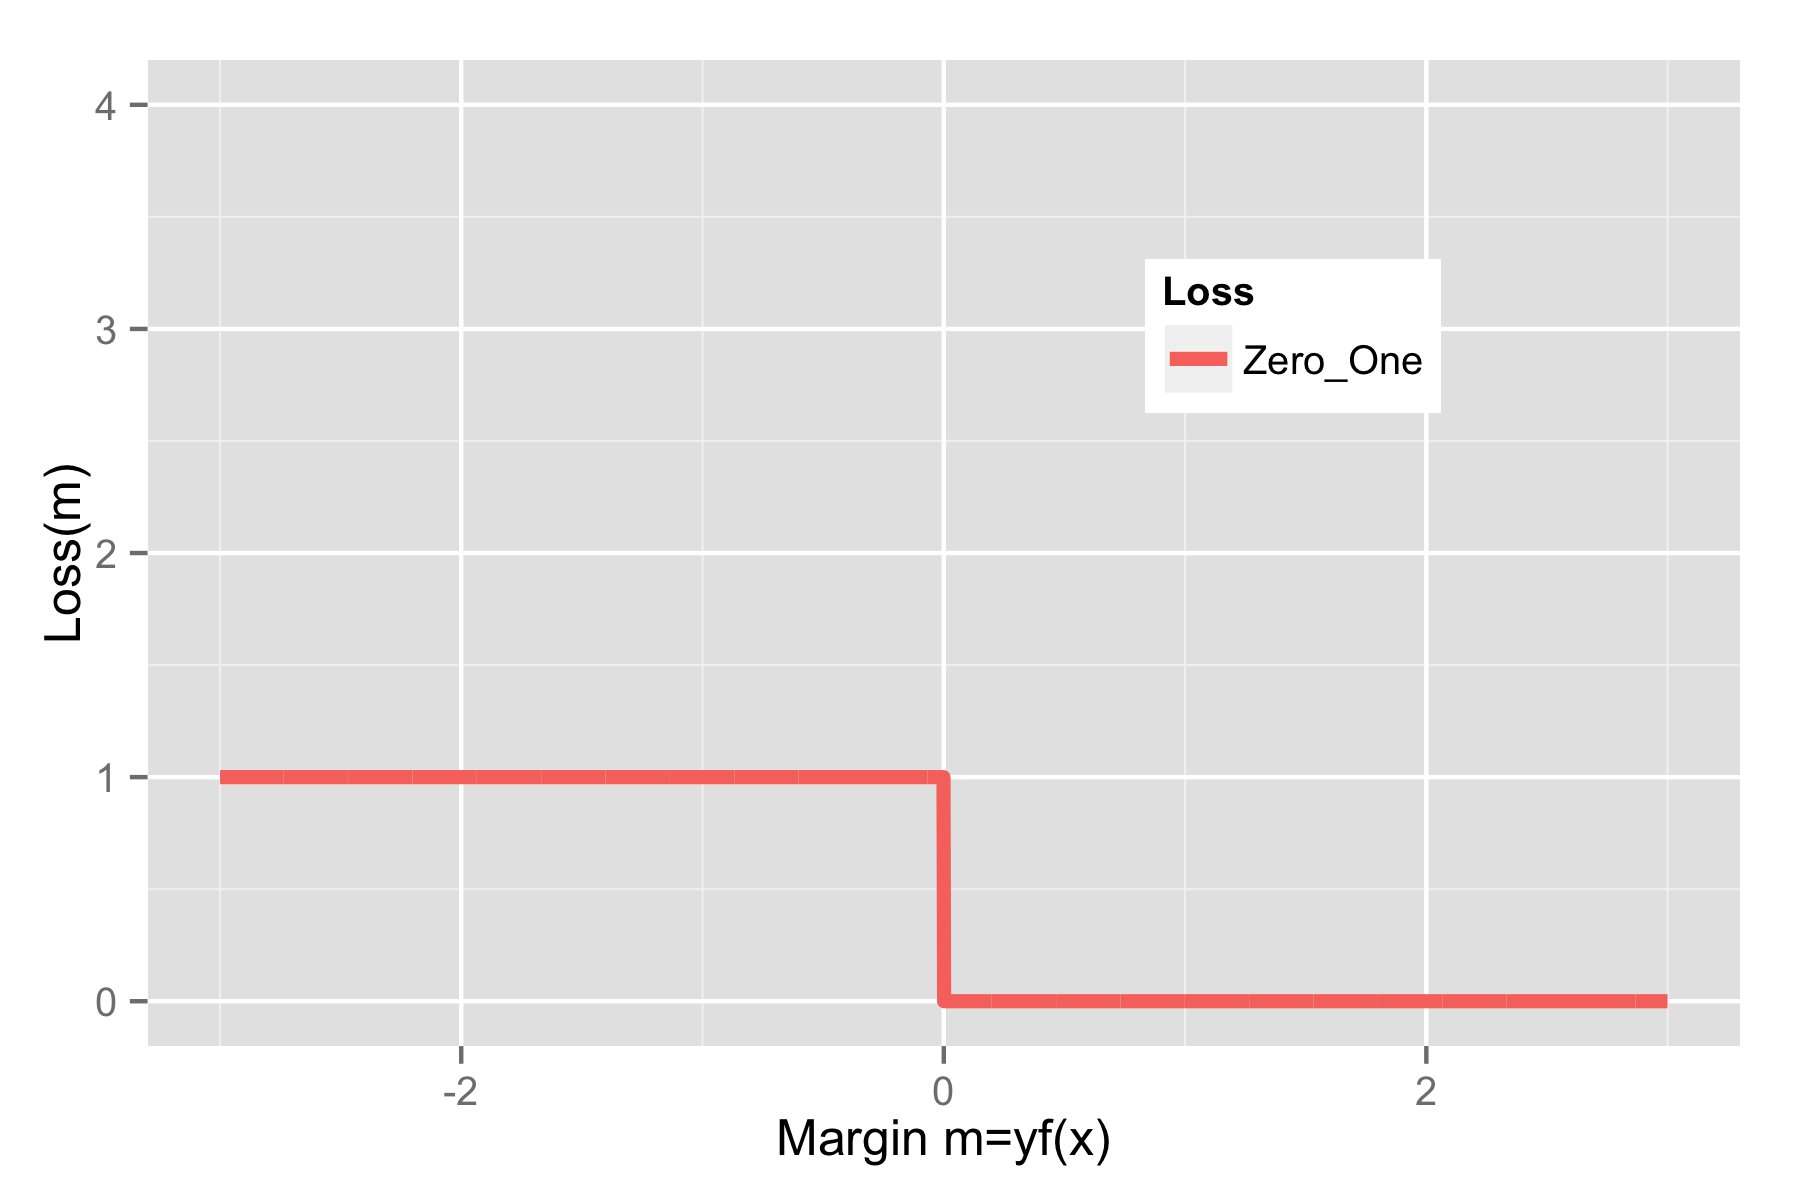
\includegraphics[height=0.6\textheight]{figures/loss.Zero_One}
\par\end{center}
\begin{itemize}
\item x-axis is \textbf{margin}: $m>0\iff\text{correct classification}$
\end{itemize}

\end{frame}

\begin{frame}{Classification Losses}

SVM/Hinge loss: $\loss_{\text{Hinge}}=\max\left(1-m,0\right)$
\begin{center}
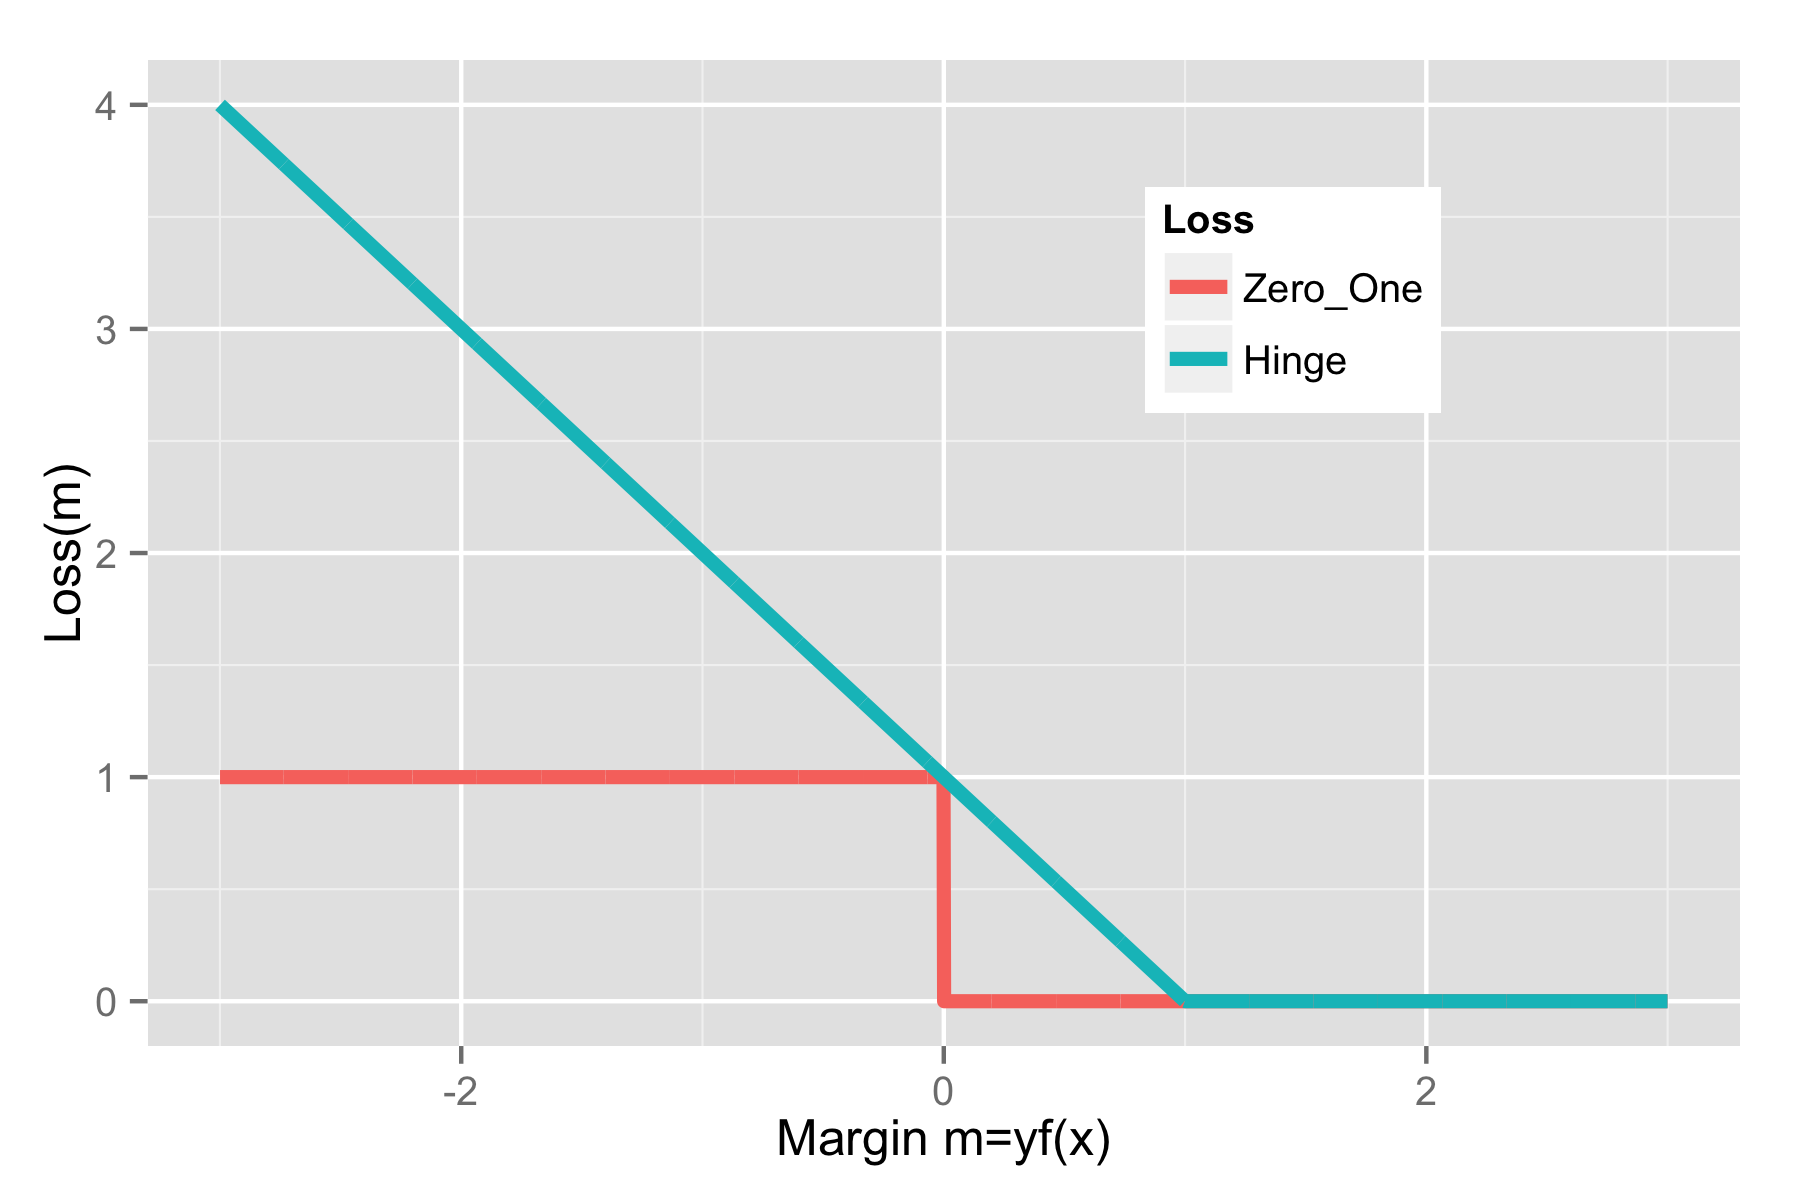
\includegraphics[height=0.6\textheight]{figures/loss.Zero_One.Hinge}
\par\end{center}

Hinge is a \textbf{convex}, \textbf{upper bound} on $0-1$ loss. Not
differentiable at $m=1$.
%We have a \textbf{``margin error''} when $m<1$.
\end{frame}

\begin{frame}{Classification Losses}

Logistic/Log loss: $\loss_{\text{Logistic}}=\log\left(1+e^{-m}\right)$
\begin{center}
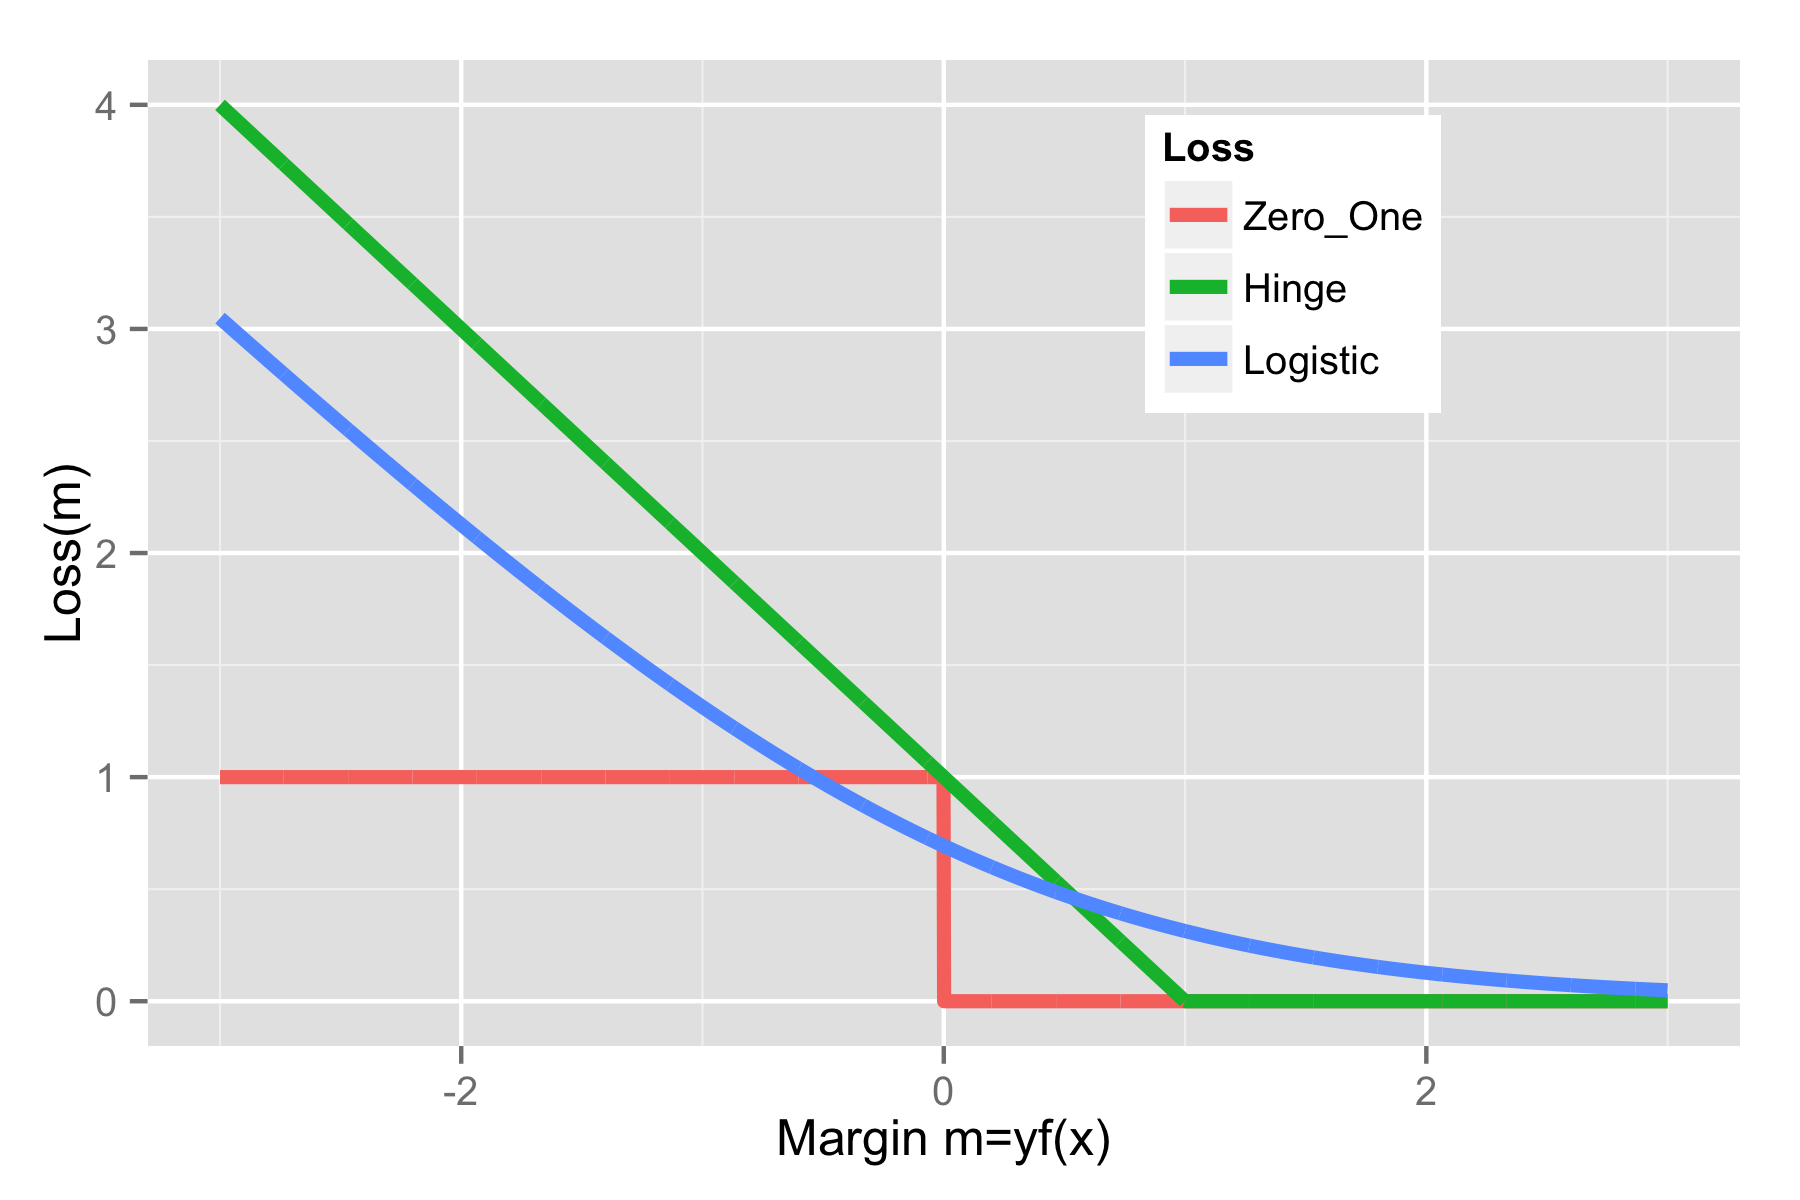
\includegraphics[height=0.6\textheight]{figures/loss.Zero_One.Hinge.Logistic}
\par\end{center}

Logistic loss is differentiable. Logistic loss always wants more margin
(loss never 0).
\end{frame}

\begin{frame}{What About Square Loss for Classification?}
\begin{itemize}
\item Action space $\ca=\reals\qquad$Output space $\cy=\left\{ -1,1\right\} $
\item Loss $\ell(f(x),y)=\left(f(x)-y\right)^{2}$.

\item Turns out, can write this in terms of margin $m=f(x)y$:
\begin{eqnarray*}
\ell(f(x),y) & = & \left(f(x)-y\right)^{2}=\left(1-f(x)y\right)^{2}=\left(1-m\right)^{2}
\end{eqnarray*}
\item Prove using fact that $y^{2}=1$, since $y\in\left\{ -1,1\right\} $.
\end{itemize}
\end{frame}

\begin{frame}{What About Square Loss for Classification?}
\begin{center}
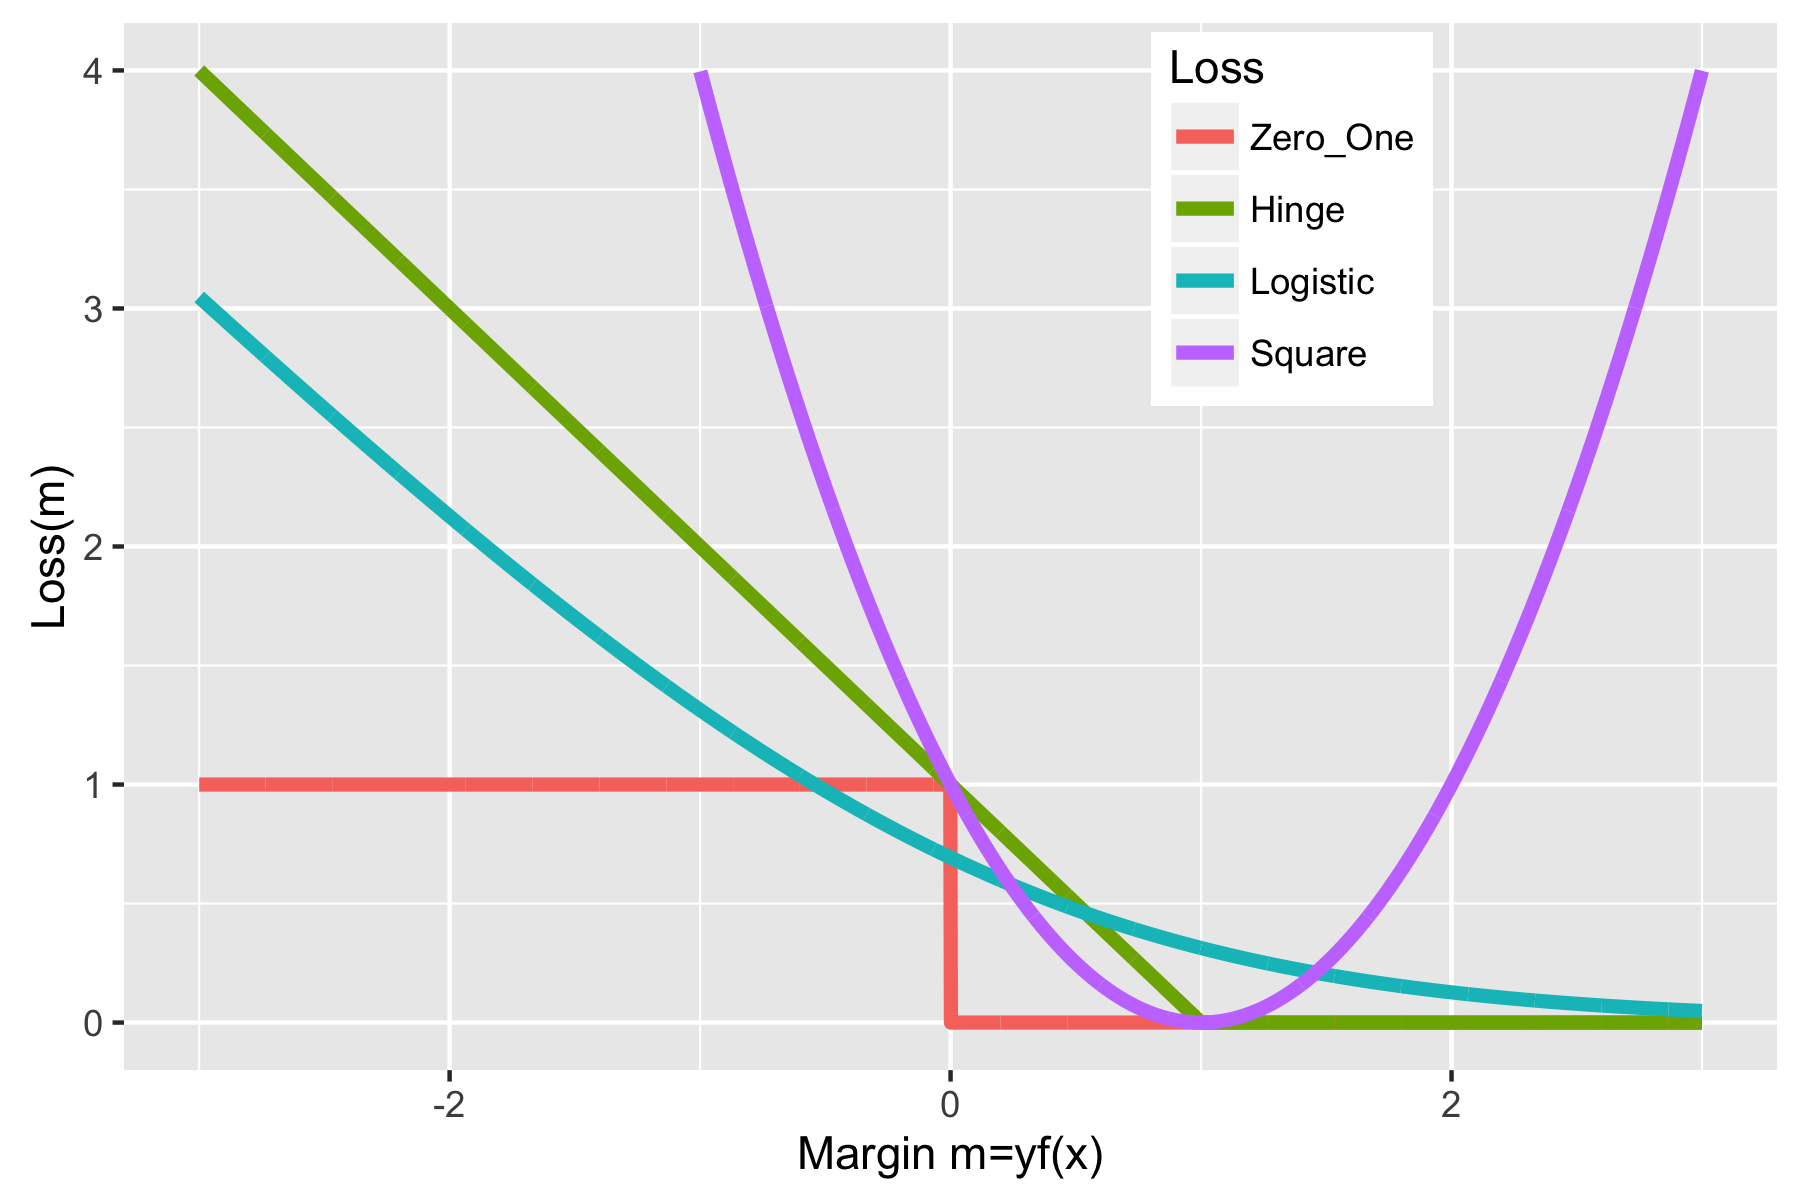
\includegraphics[height=0.6\textheight]{figures/loss.Zero_One.Hinge.Logistic.Square}
\par\end{center}

Heavily penalizes outliers (e.g. mislabeled examples).

May have higher sample complexity (i.e. needs more data) than hinge
\& logistic\footnote{{\tiny{}Rosasco et al's ``Are Loss Functions All the Same?'' \url{http://web.mit.edu/lrosasco/www/publications/loss.pdf}}}. 

\end{frame}


\end{document}
